\renewcommand*{\thefootnote}{\fnsymbol{footnote}}
\setcounter{footnote}{0}
\chapter{Study Materials for Chapter 4}
\label{app-prelim}

%\newcommand{\TODO}[1]{{\color{red}\bfseries [[TODO: #1]]}}
\newcommand{\todo}[1]{{\color{red}\bfseries [[TODO: #1]]}}

\hyphenation{retro-active-ly recommend-ation}

\newcommand\insight[1]{
	\noindent 
	\fcolorbox{gray!20}{gray!20}{
		\parbox{0.92\columnwidth}
		{#1}
		\hspace*{0.5ex}
	}
}

\newcommand{\tooltwo}{\texttt{class-bot}\xspace}
\newcommand{\toolone}{\texttt{tool-recommender-bot}\xspace}

\newcommand{\tele}{naive \textit{telemarketer design}\xspace}
\newcommand{\TELE}{Naive \textit{Telemarketer Design}\xspace}
\newcommand{\suggs}{GitHub \textsl{suggested changes}\xspace}
\newcommand{\sugg}{\textsl{suggested changes}\xspace}
\newcommand{\SUGGS}{GitHub \textsl{Suggested Changes}\xspace}
\newcommand{\suggtag}{\texttt{\`\`\`~\texttt{suggestion}}\xspace}
\newcommand{\fence}{\texttt{\`\`\`}\xspace}
\newcommand{\ep}{\textsc{Error Prone}\xspace}
\newcommand{\EP}{\textsc{Error Prone}\xspace}
\newcommand{\pom}{\textit{pom.xml}\xspace}
\newcommand{\PEP}{\texttt{PEP 3105}\xspace}
\newcommand{\ser}{R}
\newcommand{\see}{C}


\newcommand{\framework}{\textsl{developer recommendation choice architectures}\xspace}
\newcommand{\Framework}{\textsl{Developer recommendation choice architectures}\xspace}
\newcommand{\FrameWork}{\textsl{Developer Recommendation Choice Architectures}\xspace}
\newcommand{\FRAMEWORK}{\textbf{\em developer recommendation choice architectures}\xspace}

\newcommand{\thesis}{\insight{By incorporating \FRAMEWORK into recommendations for software engineers, we can \textbf{\em nudge} developers to adopt behaviors useful for improving code quality and developer productivity.}}


\section{\em ``How Software Users Recommend Tools to Each Other''}
\label{app-peer}

% \subsection{Data}

% The dataset participants analyzed to complete the tasks is available online.\footnote{https://www.kaggle.com/c/titanic/data}

\subsection{Study Script}
\label{app-peer-tasks}

\subsubsection*{\large Pre Task:} 

The dataset is picked from kaggle.com’s Titanic competition: 

\url{https://www.kaggle.com/c/titanic} \\

\noindent
The Variable descriptions are given here: 

\url{https://www.kaggle.com/c/titanic/data} \\

\noindent
Answer any questions about the dataset. \\

\noindent
Please do not use the internet to answer the questions. \\

\noindent
Please work on the tasks together in pairs.   \\

\noindent
The time to spend on the task is 60 mins, which comes to 7 to 8 mins on each task. However, this is just a recommendation. 
(the participants were asked to do their best when answering the questions and not to bother about the time etc. ) \\

\noindent
Please use any tool you are comfortable with to answer these questions. This computer has Excel, Rstudio, Python, SAS JMP Pro 12, and MySQL Workbench. If you need anything else, we can download that as well.  \\

\noindent
\textbf{The total time for the task is 60 mins. Please do not spend more than 45 mins in the training tasks which comes to around 7 to 8 mins on each question.} 

\subsubsection*{\large Tasks:}

\textbf{Student Task}

\noindent
Task: For a to e, please to describe the relationship. For f the factors should be ranked from the most significant to least significant. You can use mean, mode, etc. to explain the ranking. \\

\noindent
\textbf{Using training data: (45 mins)}
\begin{itemize}
    \item[a.] What is the relationship between the (gender, age) and number of sibling/spouse (SibSp) traveling? 
    \item[b.] What is the  relationship between the Title(you can find this in the name) and the number of children/parents (Parch) traveling? 
    \item[c.] What is the relationship between the Title(you can find this in the name) and the age and gender? 
    \item[d.] What is the relationship between (class, fair) and age? 
    \item[e.] What is the relationship between (the fare and class) and the city embarked? 
    \item[f.] Please rank all the factors (a-e) for their contribution to survival. The factors should be ranked from the most significant to least significant. You can use mean, mode, etc. to explain the ranking.
\end{itemize}

\noindent
\textbf{On the testing data: (10 mins)}

Please find whether these people survived.

\begin{itemize}
    \item[a.] Chaffee, Mrs. Herbert Fuller (Carrie Constance Toogood)
    \item[b.] Robins, Mr. Alexander A
    \item[c.] Peltomaki, Mr. Nikolai Johannes 
    \item[d.] Abelseth, Mr. Olaus Jorgensen
    \item[e.] Mulvihill, Miss. Bertha E
    \item[f.] Thomas, Mr. John
    \item[g.] Daniels, Miss. Sarah
    \item[h.] Delalic, Mr. Redjo
\end{itemize}

\noindent
\textbf{LAS Analyst Task}

\noindent
Task: For a to c, please describe the relationship between the categories. For d the factors should be ranked from the most significant to least significant. You can use mean, mode, etc. to explain the ranking. \\

\noindent
\textbf{Using train.csv: (35 mins)}
\begin{itemize}
    \item[a.] What is the relationship between the gender (Sex), age, and the number of siblings/spouse traveling (SibSp)? 
    \item[b.] What is the relationship between the Title (you can find this in the name- Mr., Mrs., Ms., Miss., Master., Dr.,  etc. There may be more than this) and the number of children/parents (Parch) traveling?
    \item[c.] What is the relationship between the fare, class (Pclass), and age? 
    \item[d.] Rank the factors for their contribution to survival. The factors should be ranked from the most significant to least significant. You can use any methods to explain the ranking. (1 = survived, 0 = died)
\end{itemize}
   

When you are comfortable with your answers to the tasks above or time is running out, please move on to the final task. Again, you must work together in pairs and you may not use the internet to answer the questions. \\

\noindent
\textbf{Using test.csv and your results from the previous task: (10 min.)}

Predict whether the following passengers survived:

\begin{itemize}
    \item[a.] Chaffee, Mrs. Herbert Fuller (Carrie Constance Toogood)
    \item[b.] Robins, Mr. Alexander A
    \item[c.] Peltomaki, Mr. Nikolai Johannes 
    \item[d.] Abelseth, Mr. Olaus Jorgensen
    \item[e.] Mulvihill, Miss. Bertha E
    \item[f.] Thomas, Mr. John
    \item[g.] Daniels, Miss. Sarah
    \item[h.] Delalic, Mr. Redjo
\end{itemize}


\subsubsection*{\large Post Task:} 

For the tasks you just completed, I’m interested in when you recommended a tool or program feature to complete the tasks. I noticed the following recommendations you made; let’s look back at them briefly. 
\textit{Open recommendation sheets.}

Do you recall making any other recommendations that I didn't write down, especially ones where help was not specifically asked for? \textit{Write them down.}

Now, let’s go through each one. May I turn on my audio recorder? \textit{Turn it on. Fill in interview portion.}


\subsection{Recommendation Sheet}

The following text was used by the researchers to track instances of peer interactions during the study sessions and to guide the discussion in the semi-structured interviews at the end of the tasks: \\

\noindent
\textbf{\Large Recommendation Sheet} \\

\textbf{Observation Data}

Person making the recommendation:  \_\_\_\_\_\_\_\_\_\_\_\_\_\_\_\_\_\_\_\_\_\_\_

Approximate time recommendation made:  \_\_\_\_\_\_\_\_\_\_\_\_\_\_\_\_\_

Tool recommended \_\_\_\_\_\_\_\_\_\_\_\_\_\_\_\_\_\_\_\_ \\

\subsection{Interview Data}
\label{app-peer-interview}

\noindent
\textbf{Semi-structured}

\noindent
\~One effective and one ineffective tool recommendation

\noindent
Previous experience with tool of choice?

\noindent
For person making the recommendation:

\begin{itemize}
    \item Why did you decide to make this recommendation?
    \item Why did you make it this way? 
    \item Why did you phrase it this way?
    \item Why did you make it at this time?
    \item Did the recomendee react in the way you expected?
    \item Anything else we should know about this?
\end{itemize}

\noindent
For person who received the recommendation:
\begin{itemize}
    \item What did you think when you got the recommendation?
    \item How helpful was the recommendation for the task you were doing? For future tasks?
    \item How helpful was the timing of the recommendation?
    \item How disruptive was the timing of the recommendation?
    \item Anything else we should know about this?
\end{itemize}

\subsection{Interaction Data List}
\label{app-peer-data}

For each recommendation observed in our study, we collected:

\begin{itemize}[topsep=0pt,itemsep=-1ex,partopsep=1ex,parsep=1ex]
    \item the type of peer interaction (Peer Observation or Peer Recommendation),
    \item the approximate time in the video the recommendation took place,
    \item which participants are the driver and navigator,
    \item the study task,
    \item the method of the driver and navigator (if possible),
    \item the name and type of the recommended feature,
    \item a transcript of the dialogue concerning the new tool,
    \item the reaction of the recommendee,
    \item instances in the study where the tool was re-used,
    \item instances where the tool was ignored for a less efficient method,
    \item the effectiveness, politeness, persuasiveness, and receptiveness scores, 
    \item whether the recommendations was under time pressure, and
    \item if the recommendation was discussed during the interview and time of discussion in the video.
\end{itemize}

\subsection{Peer Interaction Characteristic Scoring}
\label{app-peer-scoring}

This section of the appendix presents the final set of criteria that the two independent researchers agreed upon for Politeness, Persuasiveness, and Receptiveness. We specifically searched for the following when analyzing the study videos and scoring these characteristics for peer interactions. \\

\noindent
\textbf{\underline{Politeness}}

\noindent
\textbf{Tact}\\
\textbf{+1} Recommender provides beneficial reason for using tool \\
\textbf{0}  No statement on advantages or disadvantages of tool \\
\textbf{-1} Recommender notes weakness of using suggested tool \\

\noindent
\textbf{Generosity} \\
\textbf{+1} Recommender offers to do the work for the recommendee \\
\textbf{0}  No statement on either peer doing work \\
\textbf{-1} Recommender makes partner complete all the work \\

\noindent
\textbf{Approbation} \\
\textbf{+1} Recommender praises or compliments partner \\
\textbf{0}  No statements of praise or insults \\
\textbf{-1} Recommender insults or offends partner \\

\noindent
\textbf{Modesty} \\
\textbf{+1} Recommender expresses humility in knowledge or abilities\\
\textbf{0}  No statements of humility or arrogance \\
\textbf{-1} Recommender praises their own knowledge or abilities \\

\noindent
\textbf{Agreement}\\
\textbf{+1} Recommender agrees with statements made by partner or uses inclusive language\\
\textbf{0}  No statements of agreement or disagreement\\
\textbf{-1} Recommender disagrees or argues with partner\\

\noindent
\textbf{Sympathy} \\
\textbf{+1} Recommender expresses congratulations, commiseration, or expresses condolences \\
\textbf{ 0}   No statements regarding sympathy or apathy \\
\textbf{-1} Recommender incites conflict, expresses dismissiveness, or enjoys pain of partner \\

\noindent
\textbf{\underline{Persuasiveness}}\\
\noindent
\textbf{Content} \\
\textbf{+1} Recommender explicitly explains why the tool suits the purpose by citing a source, relating to previous experience, explaining how it works, or presenting why it's useful  \\
\textbf{-1} Recommender does not provide any information explaining why to use the suggested tool \\

\noindent
\textbf{Structure} \\
\textbf{+1} Recommender presents the tool before explaining why it should be used \\
\textbf{-1} Recommender explains why a tool should be used before saying the tool or does not provide content \\

\noindent
\textbf{Style}
\textbf{+1} Recommender avoids hedging, hesitating, recommending multiple features simultaneously, asking if a tool should be used, tag questions, and passive and powerless language (i.e. ``I think'', ``I guess'', ``sort of'', excessive number of ``Uh...'', etc.) \\
\textbf{-1} Recommender uses the statements above in their recommendation\\

\noindent
\textbf{\underline{Receptiveness}} \\
\textbf{Demonstrate Desire} \\
\textbf{+1} Recommendee explicitly expresses interest or asks questions to learn more information about tool \\
\textbf{0}  No statements demonstrating desire \\
\textbf{-1} Recommendee explicitly expresses disinterest in using tool \\

\noindent
\textbf{Familiarity}\\
\textbf{+1} Recommendee explicitly expresses familiarity with tool and environment or compares to a familiar tool \\
\textbf{0}  No statements on familiarity \\
\textbf{-1} Recommendee explicitly states they are unfamiliar with the tool or environment \\


\subsection{Demographics Questionnaire}
\label{app-peer-survey}

\begin{enumerate}
    \item Gender: \_\_\_\_\_\_\_\_\_\_\_\_
    \item Occupation: \_\_\_\_\_\_\_\_\_
    \item What is your major (or speciality of highest degree earned)? \_\_\_\_\_\_\_\_\_
    \item How many years have you known your group member? \_\_\_\_\_\_
    How would you describe your relationship with your partner? (Check all that apply)
    \begin{itemize}
        \item[a.] Professional \_\_\_
        \item[b.] Personal \_\_\_
        \item[c.] Academic \_\_\_
        \item[d.] None \_\_\_
    \end{itemize}
    \item What software do you know your partner uses regularly? \\ \_\_\_\_\_\_\_\_\_\_\_\_\_\_\_\_\_\_\_\_\_\_\_\_\_\_\_\_\_\_\_\_\_\_\_\_\_\_\_\_\_\_\_\_\_
    \item Have you and your partner worked together in some capacity in the past? \_\_\_\_\_\_\_\_\_\_\_\_\_\_\_\_\_\_
    \begin{itemize}
        \item[a.] If Yes, please describe any computer-based work you have done together: \\
        \_\_\_\_\_\_\_\_\_\_\_\_\_\_\_\_\_\_\_\_\_\_\_\_\_\_\_\_\_\_\_\_\_\_\_\_\_\_\_\_\_\_\_\_\_
    \end{itemize}
    \item How many years of experience do you have with the software(s) your group used to complete the tasks? \_\_\_\_\_\_\_\_\_\_\_\_\_\_\_\_\_\_\_\_\_\_\_\_\_\_\_\_\_\_\_\_\_\_\_\_\_\_\_\_\_\_\_\_\_
\end{enumerate}

\subsection{Participants}
\label{app-peer-participants}

\begin{table}[H]
	\caption{Peer Interaction Study Participants}
	\centering
	\begin{tabular}{lll}
		\hline
		\textbf{Participant} & \textbf{Gender} & \textbf{Major} \\
		\hline
		S1 & Male & Industrial Engineering $   $ $\blacklozenge$\\
		S2 & Male & Computer Science $   $ $\blacklozenge$\\
		%\hline
		S3 & Male & Computer Science $   $ $\blacklozenge$\\
		S4 & Male & Computer Science $   $ $\blacklozenge$\\
		%\hline
		S5 & Male & Computer Science $   $ $\blacklozenge$\\
		S6 & Male & Computer Science $   $ $\blacklozenge$\\
		%\hline
		S7 & Male & Computer Science $   $ $\blacklozenge$\\
		S8 & Male & Computer Science $   $ $\blacklozenge$\\
		%\hline
		S9 & Male & Industrial Engineering $   $ $\blacklozenge$\\
		S10 & Female & Computer Science $   $ $\blacklozenge$\\
		%\hline
		S11 & Female & Biochemistry $   $ $\blacklozenge$\\
		S12 & Female & Biochemistry $   $ $\lozenge$\\
		%\hline
		S13 & Female&Computer Science$   $ $\blacklozenge$\\
		S14 & Male & Computer Science $   $ $\blacklozenge$\\
		\hline \\
		\end{tabular}
	
		\begin{tabular}{lll}
		\hline 
		\textbf{Participant} & \textbf{Gender} & \textbf{Position} \\
		\hline
		L1 & Female & Researcher 
\includegraphics[height=1em]{Chapter-3/images/hands.png} \\
		L2 & Female & Researcher 
\includegraphics[height=1em]{Chapter-3/images/hands.png} \\
		%\hline
		L3 & Male & Program Manager 
\includegraphics[height=1em]{Chapter-3/images/hands.png} 
\includegraphics[height=1em]{Chapter-3/images/computer.png} \\
		L4 &Female&Director of Operations 
\includegraphics[height=1em]{Chapter-3/images/hands.png} 
\includegraphics[height=1em]{Chapter-3/images/computer.png} \\
		%\hline
		L5 & Male &Researcher, Analyst \\
		L6 & Male & Computer Engineer \\
		%\hline
		L7 & Female & Researcher \\ 
		L8 & Male & Language Analyst \\
		%\hline
		L9 & Female & Engineer 
\includegraphics[height=1em]{Chapter-3/images/hands.png} 
\includegraphics[height=1em]{Chapter-3/images/computer.png} \\
		L10 & Female & Engineer 
\includegraphics[height=1em]{Chapter-3/images/hands.png} 
\includegraphics[height=1em]{Chapter-3/images/computer.png} \\
		%\hline
		L11 & Female & Intel Analyst, Researcher 
\includegraphics[height=1em]{Chapter-3/images/hands.png} \\
		L12 & Male & Systems Researcher 
\includegraphics[height=1em]{Chapter-3/images/hands.png} \\
	\hline
	\end{tabular}
    {\footnotesize
	\begin{itemize}[topsep=0pt,itemsep=-1ex,partopsep=1ex,parsep=1ex]
	\centering
        \item[] $\blacklozenge$ Graduate Student $     $ $\lozenge$ Undergraduate Student
        \item[] 
\includegraphics[height=1em]{Chapter-3/images/hands.png} Previous relationship with partner 
        \item[] 
\includegraphics[height=1em]{Chapter-3/images/computer.png} Previously completed computer-based work with partner
    \end{itemize}
    }
	\label{tab:peer-participants}
\end{table}

\newpage

\section{\em ``Sorry to Bother You: Designing Bots for Effective Recommendations''}

\subsection{Naive Telemarketer Design}
\label{app-sorry}

\begin{figure}[H]
  \centering
  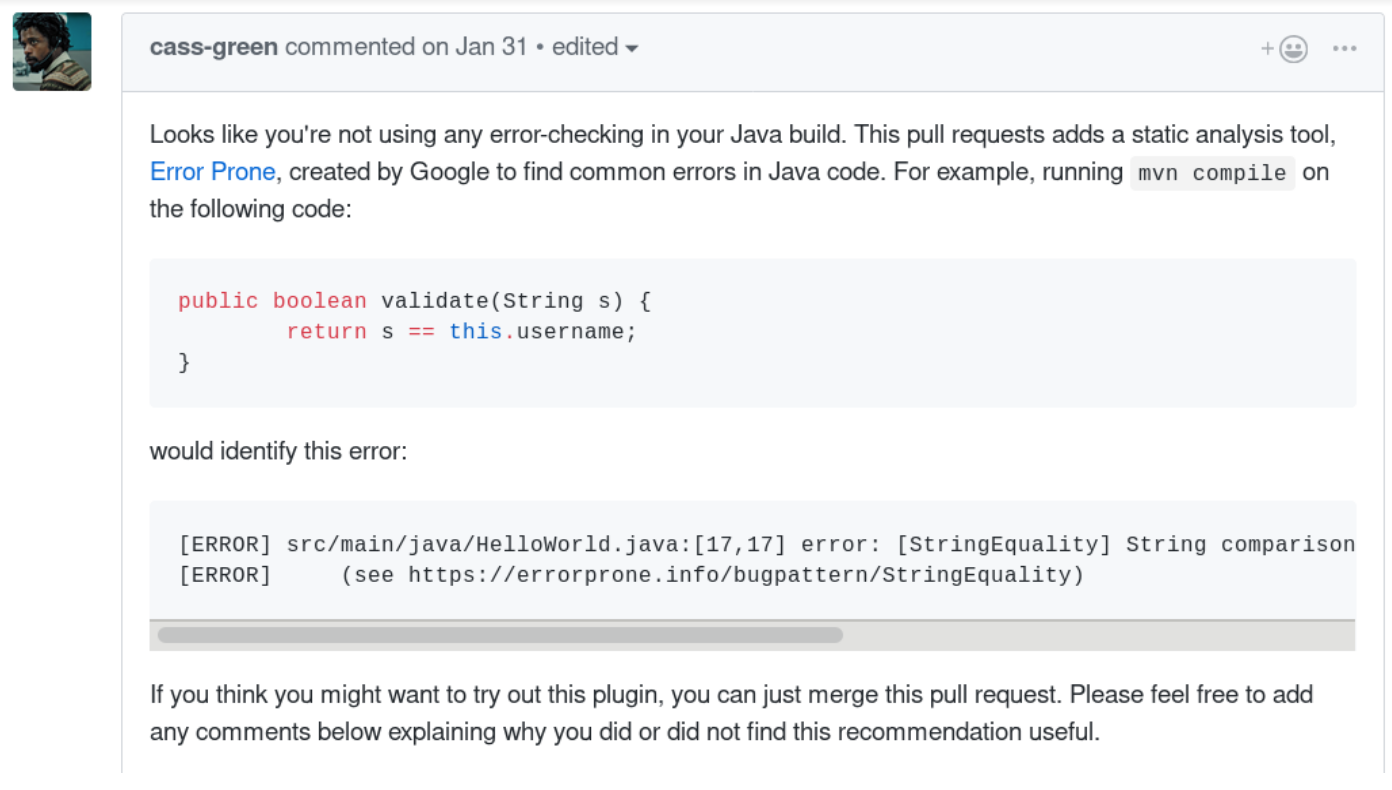
\includegraphics[width=\textwidth]{Appendix-A/images/tele.png}
  \caption{\TELE recommendation from \texttt{tool-recommender-bot}}
  \label{fig:telemarketer}
\end{figure}

\subsection{Study Projects}
\label{app-sorry-projects}

This section outlines the projects that received recommendations for the \tele study and provides the automated pull requests submitted to projects by \toolone:

\begin{enumerate}[topsep=0pt,itemsep=-1ex,partopsep=1ex,parsep=1ex]

\item \url{https://github.com/jponge/lzma-java/pull/15}
\item \url{https://github.com/fizzed/rocker/pull/102}
\item \url{https://github.com/GideonLeGrange/mikrotik-java/pull/61}
\item \url{https://github.com/Asquera/elasticsearch-http-basic/pull/70}
\item \url{https://github.com/debezium/debezium/pull/760}	
\item \url{https://github.com/dropwizard/dropwizard-elasticsearch/pull/34}
\item \url{https://github.com/Nodeclipse/nodeclipse-1/pull/229}	
\item \url{https://github.com/forge/roaster/pull/101}	
\item \url{https://github.com/recommenders/rival/pull/131}{recommenders/rival\#131}
\item \url{https://github.com/tbroyer/gwt-maven-archetypes/pull/58}
\item \url{https://github.com/Hygieia/Hygieia/pull/2696}\footnote[2]{Merged}
\item \url{https://github.com/wro4j/wro4j/pull/1069}\footnote[8]{Merged, then reverted}
\item \url{https://github.com/jplag/jplag/pull/61}
\item \url{https://github.com/gitbucket/markedj/pull/21}	
\item \url{https://github.com/jhalterman/expiringmap/pull/60}		
\item \url{https://github.com/arquillian/arquillian-core/pull/190}
\item \url{https://github.com/graphstream/gs-core/pull/305}
\item \url{https://github.com/jirutka/validator-collection/pull/27}
\item \url{https://github.com/jreijn/spring-comparing-template-engines/pull/37}
\item \url{https://github.com/elkan1788/mpsdk4j/pull/8}		
\item \url{https://github.com/arturmkrtchyan/iban4j/pull/59}	
\item \url{https://github.com/games647/LagMonitor/pull/51}	
\item \url{https://github.com/jmxtrans/jmxtrans-agent/pull/137}	
\item \url{https://github.com/fakereplace/fakereplace/pull/34}		
\item \url{https://github.com/google/binnavi/pull/113}	
\item \url{https://github.com/devnied/AndroidBitmapTransform/pull/1}
\item \url{https://github.com/ebnew/ki4so/pull/7}	
\item \url{https://github.com/bujiio/buji-pac4j/pull/83}	
\item \url{https://github.com/cathive/fx-guice/pull/26}	
\item \url{https://github.com/vvakame/JsonPullParser/pull/43}		
\item \url{https://github.com/cderoove/damp.ekeko/pull/2}	
\item \url{https://github.com/write2munish/Akka-Essentials/pull/8}
\item \url{https://github.com/Slim3/slim3/pull/30}
\item \url{https://github.com/jirutka/spring-rest-exception-handler/pull/30}
\item \url{https://github.com/yyuu/jetty-nosql-memcached/pull/35}
\item \url{https://github.com/casidiablo/persistence/pull/17}	
\item \url{https://github.com/dsyer/sparklr-boot/pull/6}	
\item \url{https://github.com/dgageot/simplelenium/pull/26}	
\item \url{https://github.com/jhalterman/concurrentunit/pull/22}	
\item \url{https://github.com/jplag/jplag/pull/62}
\item \url{https://github.com/kwart/jd-cmd/pull/19}	
\item \url{https://github.com/leveluplunch/levelup-java-examples/pull/5}
\item \url{https://github.com/ngageoint/elasticgeo/pull/97}		
\item \url{https://github.com/perfectsense/dari/pull/317}		
\item \url{https://github.com/rchodava/datamill/pull/119}		
\item \url{https://github.com/RichardWarburton/lambda-behave/pull/98}
\item \url{https://github.com/roundrop/facebook4j/pull/122}	
\item \url{https://github.com/spring-guides/tut-spring-boot-oauth2/pull/97}
\item \url{https://github.com/twitter/hbc/pull/195}	
\item \url{https://github.com/viritin/viritin/pull/362}	
\item \url{https://github.com/SINTEF-9012/JArduino/pull/82}		
\item \url{https://github.com/apache/bigtop/pull/461}
\end{enumerate}